\documentclass[solution, letterpaper]{cs121}

\usepackage{tikz-qtree}
\usepackage{graphicx}

%% Please fill in your name and collaboration statement here.
%\newcommand{\studentName}{Renzo Lucioni and Daniel Broudy}
%\newcommand{\collaborationStatement}{I collaborated with...}
\newcommand{\solncolor}{red}
\begin{document}

\header{2}{March 1, 2013, at 12:00 PM}{}{}

%%%%%%%%%%%%%%%%%%%%%%%%%%%%%%%%%%%%%%%%%%%%%%%%%%%%
\problem{9} For this problem, we assume that an image is a $3 \times 3$ array of pixels (inputs) arranged as follows:
\begin{center}
\begin{tabular}{ l c r }
  $x_1$ & $x_2$ & $x_3$ \\
  $x_4$ & $x_5$ & $x_6$ \\
  $x_7$ & $x_8$ & $x_9$ \\
\end{tabular}
\end{center}
Each $x_k$ in the input vector {\textbf{\emph{x}}} represents a pixel state, and can be either 1 (on) or 0 (off). Let the weight vector {\textbf{\emph{w}}} $= (w_0, w_1, \ldots, w_9)$ represent the weights of the corresponding inputs in the array. Let $x_0$ be the special instance that is always fixed at 1, and let $w_0$ be the threshold of the perceptron activation function. We will use the threshold activation function 
\begin{equation*}
  g(s)=\begin{cases}
    +1, & \text{if $s  >  0$}.\\
    -1, & \text{otherwise}.
  \end{cases}
\end{equation*}
where $s = {\textbf{\emph{x}}}^\top{\textbf{\emph{w}}}$ (i.e., the weighted sum of the inputs).

\subproblem Bright-or-dark: at least 75\% of the pixels are on, or at least 75\% of the pixels are off. \\

Assume for the purpose of contradiction that there exists some perceptron recognizing ``bright-or-dark" with weights {\textbf{\emph{w}}}. Say we turn off pixels $x_1$ and $x_2$ and leave the rest on. Greater than 75\% of the pixels are on, and so the perceptron outputs 1, implying that $s > 0$. That is,
\[ s = w_0 + w_3 + \ldots + w_9 > 0 \]
Say we also turn off pixel $x_3$, leaving the rest on. Now there are not 75\% of pixels on or off, and so the perceptron outputs $-1$, implying that $s \leq 0$. That is,
\[ s = w_0 + w_4 + \ldots + w_9 \leq 0 \]
The removal of $w_3$ causes $s$ to become less than or equal to 0, hence it must be that $w_3 > 0$. \\

Now we consider what happens when we turn on pixels $x_1$ and $x_2$ and leave the rest off. Greater than 75\% of the pixels are off, and so the perceptron outputs 1, implying that $s > 0$. That is,
\[ s = w_0 + w_1 + w_2 > 0 \]
Say we also turn on pixel $x_3$, leaving the rest off. Now there are not 75\% of pixels on or off, and so the perceptron outputs $-1$, implying that $s \leq 0$. That is,
\[ s = w_0 + w_1 + w_2 + w_3 \leq 0 \]
The addition of $w_3$ causes $s$ to become less than or equal to 0, hence it must be that $w_3 < 0$. But this is a contradiction, since it cannot be that $w_3 > 0$ and $w_3 < 0$. Therefore, there exists no perceptron recognizing ``bright-or-dark."

\subproblem Top-bright: a larger fraction of pixels is on in the top row than in the bottom two rows. \\

Let pixels $x_1, x_2,$ and $x_3$ represent the top row, and let the rest of the pixels in the array represent the bottom two rows. A perceptron recognizing ``top-bright" is defined by the set of weights {\textbf{\emph{w}}} such that $w_0 = 0$, $w_1 = w_2 = w_3 = \frac{1}{3}$ and $w_4 = w_5 = w_6 = w_7 = w_8 = w_9 = -\frac{1}{6}$. We observe that our perceptron outputs 1 only when a larger fraction of pixels is on in the top row than in the bottom two rows, since $s > 0$ only when this is the case.

\subproblem Connected: the set of pixels that are on is connected. \\

Assume for the purpose of contradiction that there exists some perceptron recognizing ``connected" with weights {\textbf{\emph{w}}}. Say we turn all pixels in the array on. The resulting image is connected, so the perceptron outputs 1, implying that $s > 0$. That is, 
\[ s = w_0 + w_1 + \ldots + w_9 > 0 \]
Now say we turn off pixels $x_1, x_3$, and $x_5$, leaving the rest on. The resulting image is not connected, so the perceptron outputs $-1$, implying that $s \leq 0$. That is,
\[ s = w_0 + w_2 + w_4 + w_6  + w_7 + w_8 + w_9 \leq 0 \]
The removal of the sum of weights $w_1 + w_3 + w_5$ causes $s$ to become less than or equal to 0, hence it must be that $w_1 + w_3 + w_5 > 0$. \\

Now we consider what happens when we turn off pixels $x_2, x_4$, and $x_6$, turning the rest on. The resulting image is not connected, so the perceptron outputs $-1$, implying that $s \leq 0$. That is,
\[ s = w_0 + w_1 + w_3 + w_5 + w_7 + w_8 + w_9 \leq 0 \]
Say we also turn off pixels $x_1, x_3$, and $x_5$, leaving only pixels $x_7, x_8$, and $x_9$ on. The resulting image is connected, so the perceptron outputs 1, implying that $s > 0$. That is,
\[ s = w_0 + w_7 + w_8 + w_9 > 0 \]
The removal of the sum of weights $w_1 + w_3 + w_5$ causes $s$ to become greater than 0, hence it must be that $w_1 + w_3 + w_5 < 0$. But this is a contradiction, since it cannot be that $w_1 + w_3 + w_5 > 0$ and $w_1 + w_3 + w_5 < 0$. Therefore, there exists no perceptron recognizing ``connected."


%%%%%%%%%%%%%%%%%%%%%%%%%%%%%%%%%%%%%%%%%%%%%%%%%%%%
\problem{12}
\subproblem Decision trees \\

Decision trees are a poor approach to digit recognition. As we saw in lecture, groups of adjacent pixels are much more useful than single pixels when recognizing digits. That is, the relationship between attributes is significantly more important than single attribute values in the context of this task. Being a greedy algorithm, ID3 would split on single pixels and would be unable to determine which pixels are good co-predictors. This would in turn make the decision trees produced by ID3 for digit recognition blind to the relationship between pixels, and therefore useless. What is more, decision trees produced by ID3 for this task would be enormous, since it is highly unlikely that a handful of single pixels could determine the label of an image, especially considering the slight variability in orientation and size present in the image data. In addition, these large decision trees would be susceptible to overfitting.

\subproblem Boosted decision stumps \\

Boosted decision stumps are also a poor approach to digit recognition. Decision stumps applied in the context of digit recognition would only split on a single pixel, making them too weak as base learners for reasons described above (i.e., it is unlikely that a single pixel could determine the label of an image, and even more so considering the slight variability in orientation and size present in the image data). That said, this approach might perform reasonably well with some data preprocessing to extract higher level features from the images such as the number of loops or edges.

\subproblem Perceptrons \\

Perceptrons are a better approach to digit recognition than decision trees or boosted decision stumps. We could assign each perceptron to learning one of the digits $0$ through $9$, then use a set of 10 perceptrons to recognize all of the digits. Each perceptron would learn to recognize its digit by making use of all pixels in the image; this is key to digit recognition because most pixels in an image are important when attempting to assign an accurate label, as discussed above. Assuming only slight variations in orientation and size in the image data (i.e., no severe rotations, translations, or skews), it would be reasonable to expect the same areas to be consistently light and dark for each digit. Each perceptron could learn to recognize these areas to produce an accurate label for its assigned digit. As we saw in (1), a limitation of perceptrons is their inability to recognize non-linearly separable functions like ``bright-or-dark" or ``connected."

\subproblem Multi-layer feed-forward neural networks \\

Multi-layer feed-forward neural networks are the best approach to digit recognition of those discussed here. Like perceptrons, multi-layer feed-forward neural networks are capable of making use of all pixels in an image, allowing them to learn the relationships between pixels. However, unlike perceptrons, neural networks can also use hidden layers to recognize non-linearly separable functions. This allows neural networks to recognize rotations, translations, and skews that would have defeated a perceptron. Thus, neural networks are both accurate and robust when determining the class of an input digit.

%%%%%%%%%%%%%%%%%%%%%%%%%%%%%%%%%%%%%%%%%%%%%%%%%%%%
\problem{68}

\begin{enumerate}
	\item See {\tt neural\textunderscore net\textunderscore impl.py}.
	\item See {\tt neural\textunderscore net\textunderscore impl.py}.
	\item See {\tt neural\textunderscore net\textunderscore impl.py}.
	\item See {\tt neural\textunderscore net\textunderscore impl.py}.
	\item We want to normalize the input values from [0, 255] to between 0 and 1 for two reasons. The first is to allow for uniform learning of suitable weights across different inputs. This does away with the need for one weight to be significantly different in magnitude than another weight ahead of time. The second reason for normalizing the input values is to prevent the sigmoid activation values from getting too close to 0 or 1, thereby avoiding the problem of ``stuck units" mentioned on page 1 in the Lecture 7 notes.
	\item
		\begin{enumerate}
		\item We trained simple networks over 100 epochs using several learning rates with different orders of magnitude: 1.0, 0.1, 0.01, and 0.001. The best training performance was exhibited with a learning rate of 0.1. Thus, we used a learning rate of 0.1.
		\item The requested graph is below. \\
		\includegraphics[scale=0.8]{Simple-Network-Alpha-0_1.pdf}
			\begin{enumerate}
				\item We are not in danger of overfitting by training for too many epochs. If we were in danger of overfitting, validation error would increase with more epochs as training error continued to decrease. However, our results for the network trained with a learning rate of 0.1 show that validation error decreases and then stabilizes at 0.129 as training error continues to decrease. This suggests that, at least for the range of 100 epochs we are considering, we are not in danger of overfitting. 
				\item A good number of epochs to train for is 48, since there is no significant improvement (i.e., decrease) in validation error beyond 48 epochs.
				\item It is important that we use a validation set instead of the actual test set when tuning the number of epochs because if we were to tune the number of epochs using the test set, we would be unintentionally optimizing our network for the test set. We want the network's performance on the test set to be an indicator of expected, general performance. Hence, we must keep the test set separate from the data used to train the network. In short, using the validation set to tune the number of epochs prevents us from overfitting accidentally.
			\end{enumerate}
		\item The network trained for 48 epochs and with a learning rate of 0.1 has a training performance of 0.87133333, a validation performance of 0.867, and a test performance of 0.912.
		\end{enumerate}
	\item
		\begin{enumerate}
			\item We trained networks with 15 and 30 fully connected hidden units over 100 epochs using several learning rates with different orders of magnitude: 1.0, 0.1, 0.01, and 0.001. The best training performance for the network with 15 hidden units was exhibited with a learning rate of 1.0. The best training performance for the network with 30 hidden units was exhibited with a learning rate of 0.1. Thus, we used learning rates of 1.0 and 0.1 for the networks with 15 and 30 hidden units, respectively.
			\item Our algorithm for automatically determining when to stop training makes use of the validation set and works as follows. We initialize a variable {\tt max\textunderscore perf\textunderscore validate} representing the maximum observed validation performance to 0.0. Each epoch, we compare the current validation performance to {\tt max\textunderscore perf\textunderscore validate}. We stop training if 1) the validation performance has not increased after 5 epochs, 2) the current validation performance is at least 0.05 below the maximum observed validation performance, or 3) we are still training when we reach the provided limit on the number of epochs. We decided on the thresholds governing our termination conditions by studying the performance results of the networks with 15 and 30 hidden units trained for (a).
			\item The requested graphs are below. \\
			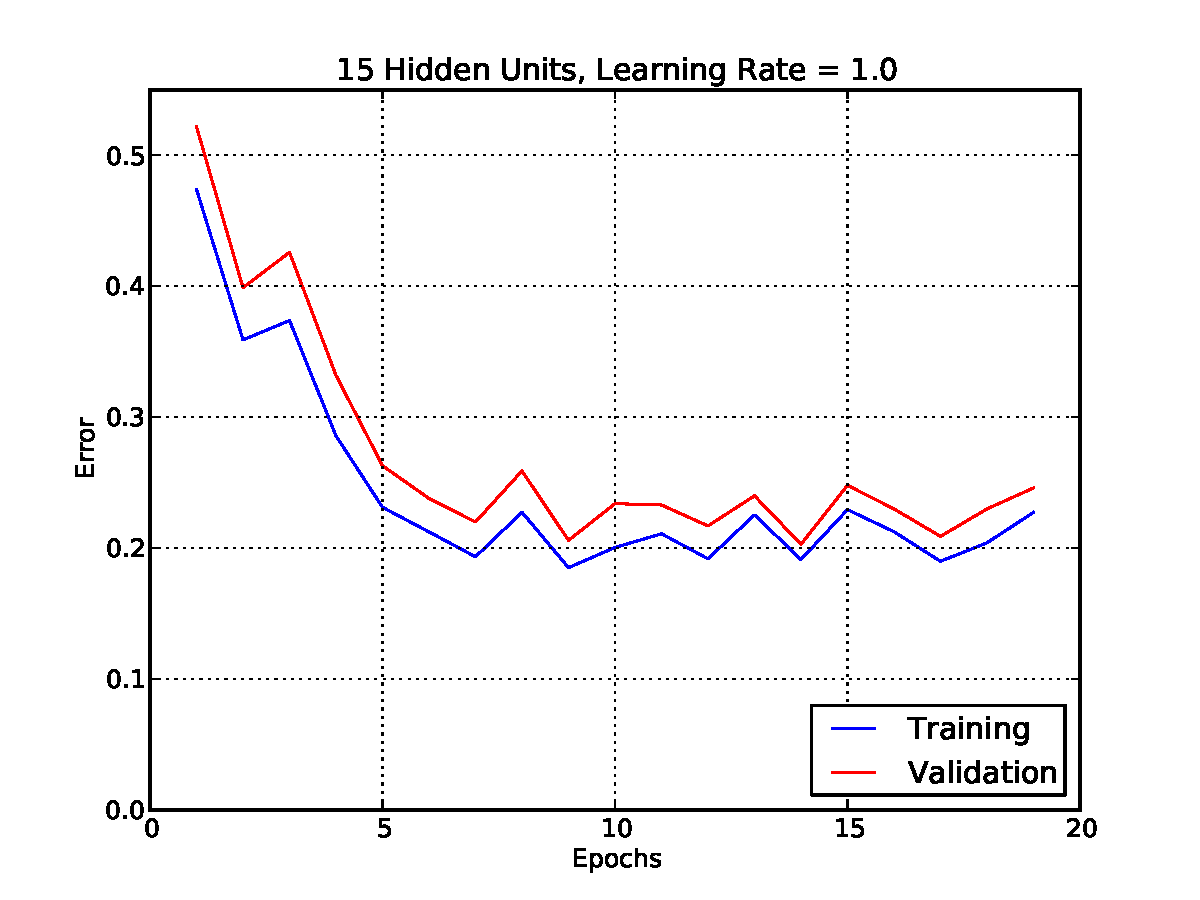
\includegraphics[scale=0.7]{15-hidden-units-alpha-1_0.pdf} \\
			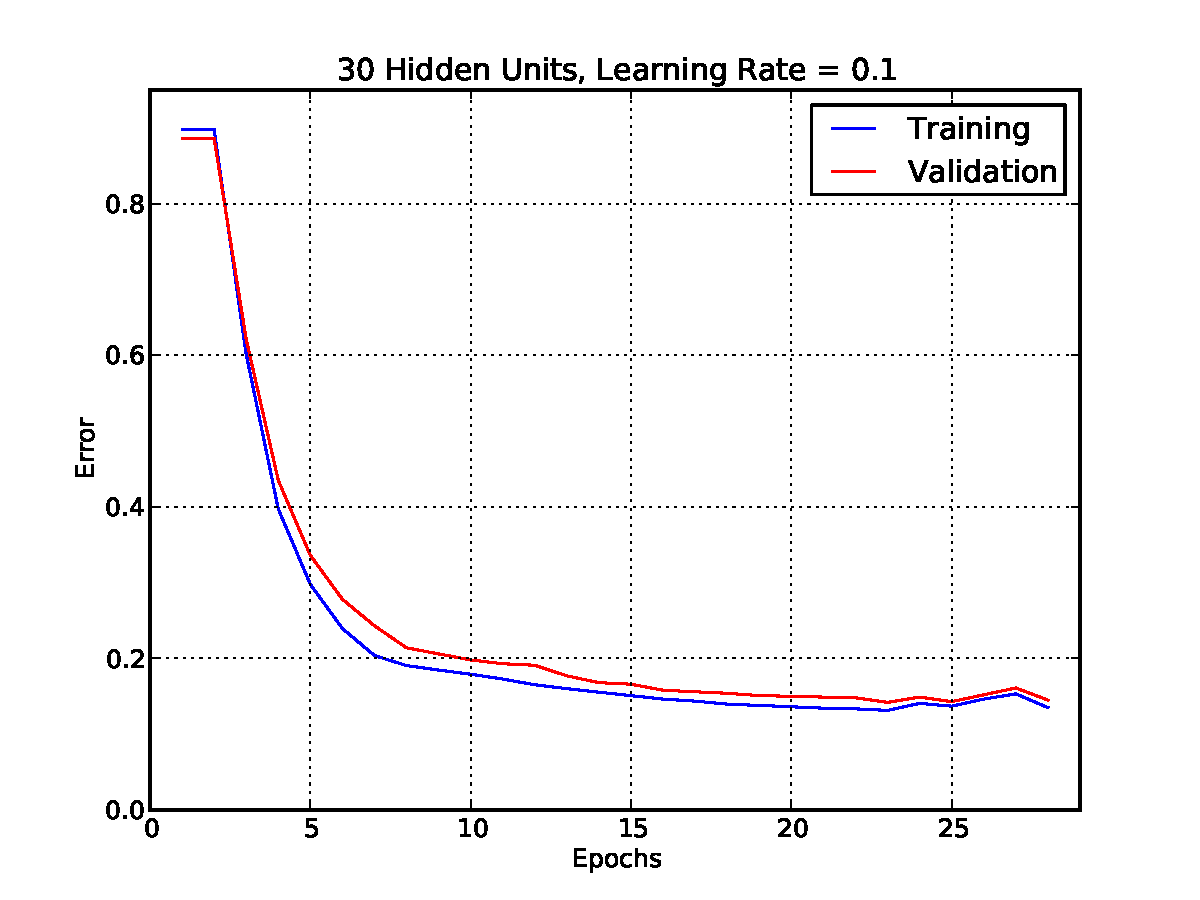
\includegraphics[scale=0.7]{30-hidden-units-alpha-0_1.pdf}
			\item Our algorithm used 19 epochs to train a network with 15 hidden units and a learning rate of 1.0, and 28 epochs to train a network with 30 hidden units and a learning rate of 0.1.
			\item Based on these experiments, we would choose the network structure with 30 hidden units. While the running time of the network structure with 30 hidden units is noticeably longer than the running time of the network structure with 15 hidden units, we note that the network with 30 hidden units has a test performance of 0.886 when trained for 28 epochs (0.907 when trained for 100 epochs) whereas the network with 15 hidden units has a test performance of 0.833 when trained for 19 epochs (0.835 when trained for 100 epochs). This is evidence that the network with 30 hidden units performs better than the network with 15 hidden units.
			\item The network with 30 hidden units, trained for 28 epochs and with a learning rate of 0.1, has a test performance of 0.886. This is slightly lower than - but on par with - the test performance of the committee of perceptrons trained for 48 epochs in part 6.
		\end{enumerate}
	\item
		\begin{enumerate}
			\item
			\item
		\end{enumerate}
\end{enumerate}

%%%%%%%%%%%%%%%%%%%%%%%%%%%%%%%%%%%%%%%%%%%%%%%%%%%%
\problem{}
%% Answer found in lecture notes 5 page 5 part e.3 Extending to Multivariate.
\begin{enumerate}
	\item We might want to use the error function $C$ to discourage the construction of an overly complicated model that is susceptible to overfitting. $C$ is trying to address the problem of assigning weights to features that are in fact irrelevant. $C$ addresses this problem by adding the second term which grows as a function of the weights in the neural network. This added term factors in the complexity of the system into the error function. By looking at all the weights, $C$ punishes the system for assigning weights to features that do not matter. The $\lambda$ factor is a regularization parameter that can be tuned to determine just how much you want the complexity to be factored into the error ($\lambda > 0$). In high-dimensional spaces, overfitting may become a problem. By extending the error function, we factor in some punishment for valuing input features that should in actuality not be weighted, discouraging complexity overall. $C$ will tend to produce sparser models, a precaution against overfitting. 
	%... It is trying to address the problem of ... It addresses this problem by ...
	\item \hfill \\
\begin{center}
%then we just take the partial derivative of this wrt w right???	
	$C({\bf w})$ = $\displaystyle\sum\limits_{n=1}^N \displaystyle\sum\limits_{j=1}^J (y_{nj} - a_{nj})^2$ +  $\lambda \displaystyle\sum\limits_{m=1}^M 
	\left(\displaystyle\sum\limits_{k=0}^K  w_{km}^2 +
	\displaystyle\sum\limits_{j=1}^J w_{mj}^2\right)$
	
\end{center}

\end{enumerate}




\end{document}



